\documentclass{article}
\usepackage[utf8]{inputenc}
\usepackage[T1]{fontenc}
\usepackage[spanish]{babel}
\usepackage{graphicx}
\usepackage{amsmath}
\usepackage{fancyhdr}
\usepackage{hyperref}
\usepackage{float}
\usepackage{geometry}

% Configuración del encabezado y pie de página
\pagestyle{fancy}
\fancyhead{}
\fancyfoot{}
\fancyfoot[C]{\thepage}
\fancyhead[L]{Tarea 1: Circuitos logicos}
\fancyhead[R]{UPIITA}
\renewcommand{\headrulewidth}{0.4pt}
\renewcommand{\footrulewidth}{0.4pt}

\title{Tarea 1: Compuerta Lógica XOR con Transistores}
\author{Marquez Sanchez Ian Jhosset \ \small 2023640691}
\date{\today}

\begin{document}

\maketitle
\thispagestyle{fancy}

\section{Resumen}
\label{sec:resumen}
En la siguiente tarea, se lleva a cabo mediante el simulador \textbf{Proteus} el diseño y simulación de una compuerta lógica \textbf{XOR} utilizando únicamente transistores. Se presenta el diseño del circuito, así como los resultados de la simulación, los cuales comprueban el funcionamiento de la compuerta y su correcta relación con su respectiva tabla de verdad.

\section{Introducción}
\label{sec:introduccion}
Para comenzar, es importante tener el conocimiento de que las compuertas \textbf{XOR} son un arreglo de otras compuertas lógicas, como las compuertas \textbf{AND} y \textbf{OR}. Estas compuertas se pueden combinar para crear el funcionamiento de la compuerta XOR, la cual presenta el funcionamiento de una suma lógica, Resultando un nivel alto solo cuando las entradas lógicas son opuestas, presentando la tabla de verdad mostrada en la figura 1. \cite{floyd2006}
\begin{figure}[H]
\centering  
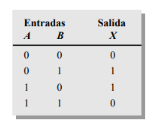
\includegraphics[width=0.5\textwidth]{IMG/TablaVerdadXOR.png}
\caption{Tabla de verdad de la compuerta XOR}
\label{fig:tabla_verdad_xor}
\end{figure}

\section{Objetivos}
\label{sec:objetivos}
\begin{itemize}
\item Diseñar el circuito de la compuerta XOR a nivel de transistores.
\item Analizar y documentar los resultados de la simulación, verificando que el circuito se comporte como una compuerta XOR.
\end{itemize}


\section{Metodología y Diseño}
\label{sec:diseno}
\subsection{Diseño del Circuito}
Se optó por diseñar la compuerta XOR utilizando transistores NPN y resistencias mediante el software \textbf{Proteus}. El diseño se basa en la combinación de dos compuertas AND y una compuerta OR, como se muestra en la figura 2.
\begin{figure}[H]
\centering
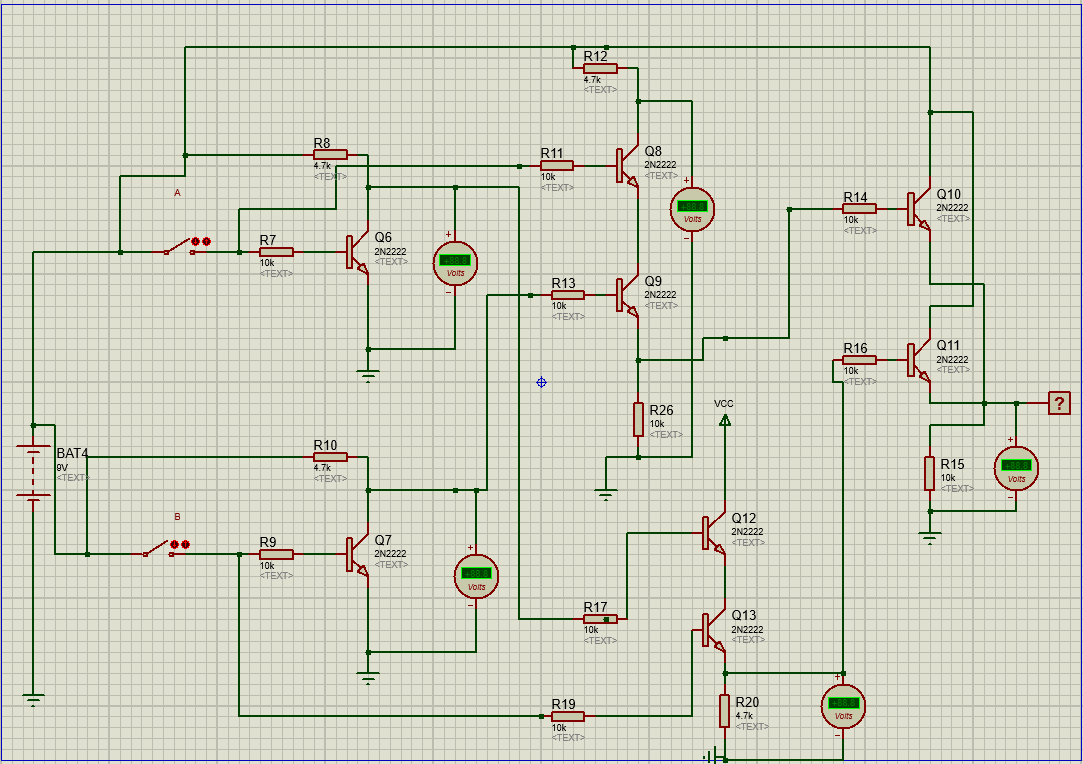
\includegraphics[width=0.8\textwidth]{IMG/DisenioCtoXor.png}
\caption{Diseño del circuito de la compuerta XOR}
\label{fig:diseño_circuito_xor}
\end{figure}

\section{Resultados de la Simulación}
\label{sec:resultados}
Comenzamos probando el circuito con diferentes combinaciones de entradas para verificar su funcionamiento. Los resultados obtenidos se compararon con la tabla de verdad de la compuerta XOR para confirmar su correcto desempeño.

\subsection{Gráficas y Evidencias}
Comenzamos con la combinación lógica A=0, B=0, obteniendo un nivel bajo en la salida. 
\begin{figure}[H]
\centering
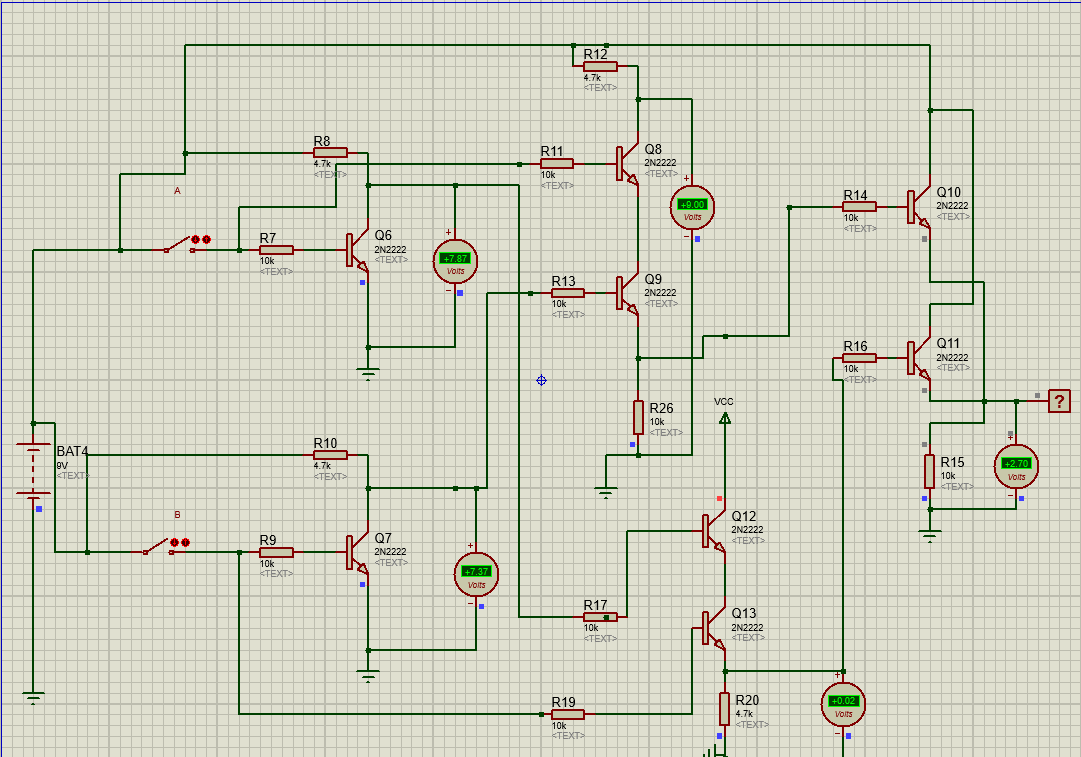
\includegraphics[width=0.8\textwidth]{IMG/00.png}
\caption{Simulación de la compuerta XOR con A=0, B=0}
\label{fig:simulacion_a0b0}
\end{figure}
Posteriormente, con A=0, B=1, la salida resultó en un nivel alto.
\begin{figure}[H]
\centering 
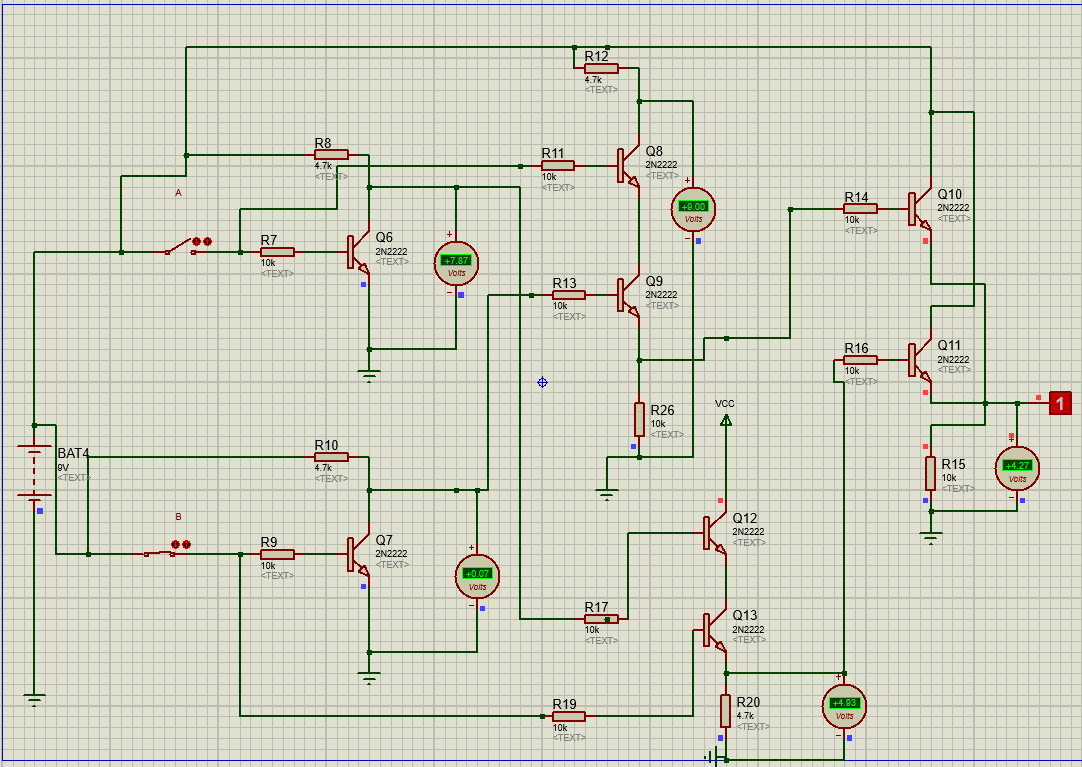
\includegraphics[width=0.8\textwidth]{IMG/01.png}
\caption{Simulación de la compuerta XOR con A=0, B=1}
\label{fig:simulacion_a0b1}
\end{figure}
Continuamos con A=1, B=0, obteniendo nuevamente un nivel alto en la salida.
\begin{figure}[H]
\centering
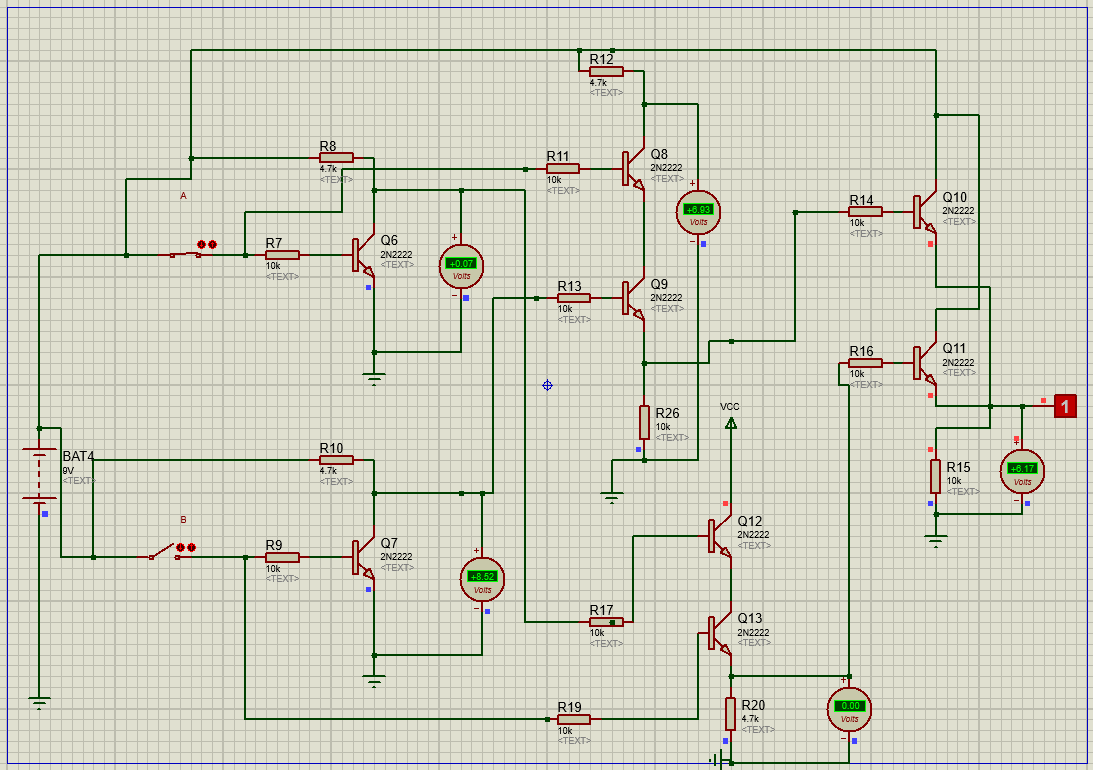
\includegraphics[width=0.8\textwidth]{IMG/10.png}
\caption{Simulación de la compuerta XOR con A=1, B=0}
\label{fig:simulacion_a1b0}
\end{figure}
Finalmente, con A=1, B=1, la salida volvió a ser un nivel bajo.
\begin{figure}[H]
\centering
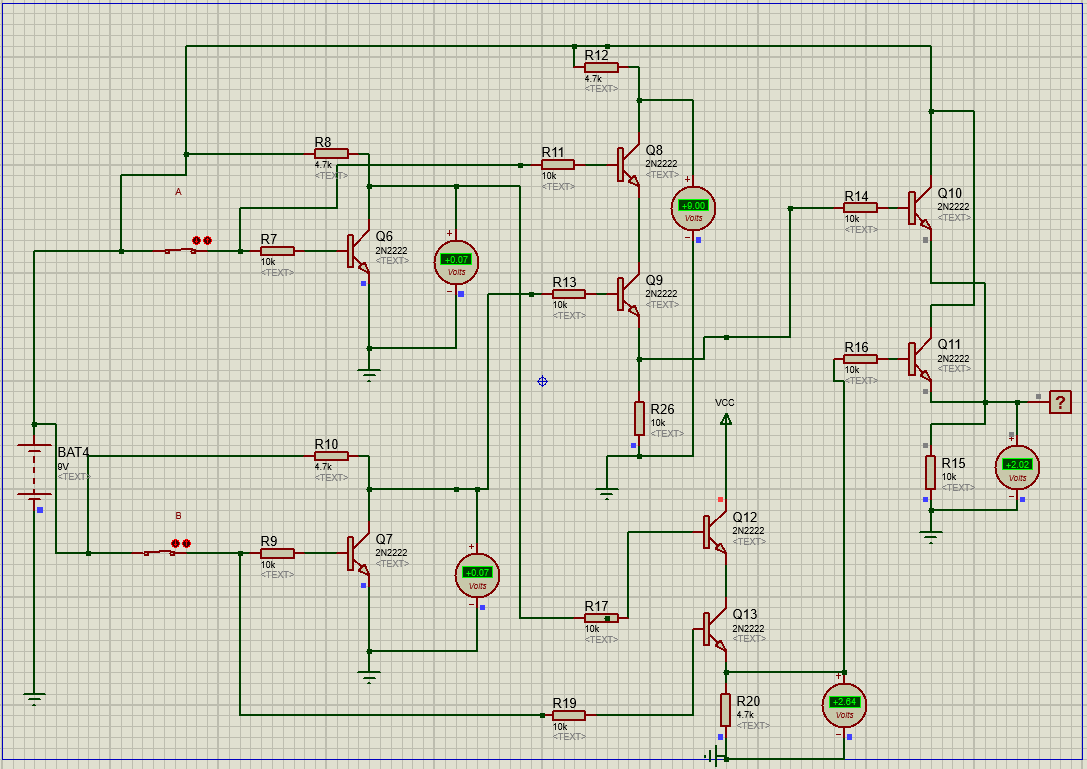
\includegraphics[width=0.8\textwidth]{IMG/11.png}
\caption{Simulación de la compuerta XOR con A=1, B=1}
\label{fig:simulacion_a1b1}
\end{figure}
Estos resultados coinciden perfectamente con la tabla de verdad de la compuerta XOR.
Sin embargo, al conectar un osciloscopio a la salida de la compuerta construida, podemos percatarnos de que, pasado un corto periodo de tiempo, el voltaje no se mantiene alto, (un si lógico), sino que cae progresivamente con el tiempo.
\begin{figure}[H]
\centering
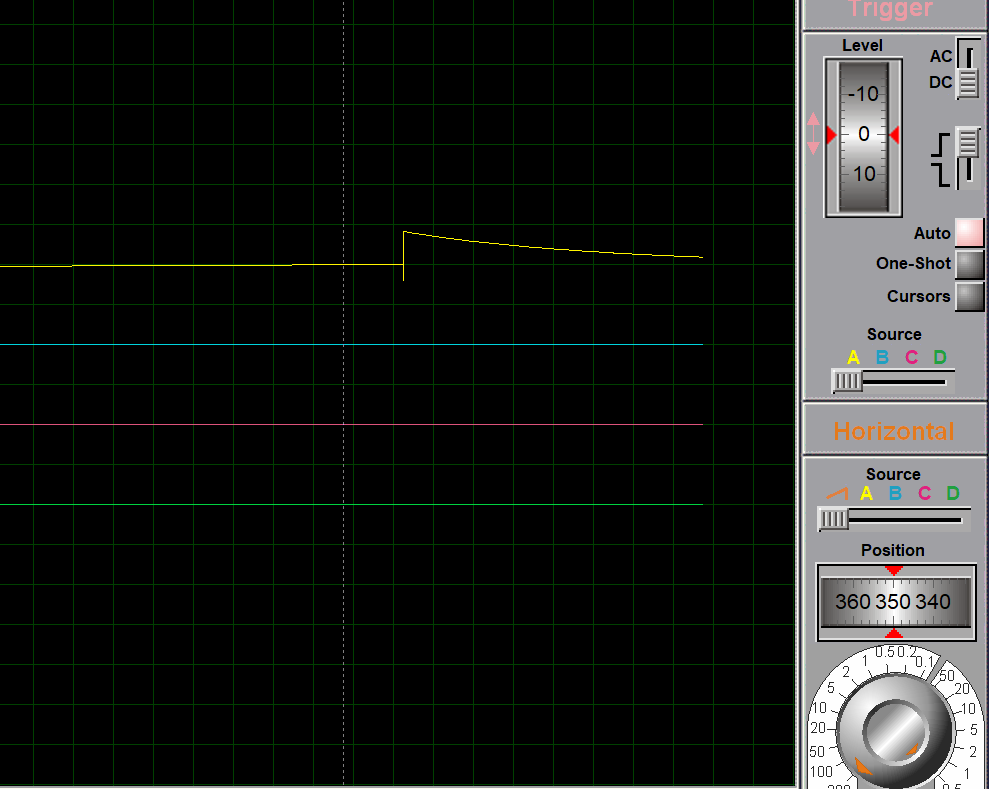
\includegraphics[width=0.8\textwidth]{IMG/Osciloscopio.png}
\caption{Salida de la compuerta XOR observada en un osciloscopio}
\label{fig:osciloscopio}
\end{figure}

\section{Conclusiones}
\label{sec:conclusiones}

Como se observa en los resultados, el circuito compuesto de transistores NPN y resistencias logra replicar el comportamiento esperado de una compuerta XOR. La simulación aproxima de una manera casi correcta el funcionamiento de una compuerta XOR, sin embargo, podemos apreciar en los voltímetros resultados que no corresponden con un comportamiento ideal de una compuerta lógica XOR, lo cual podemos atribuir al tipo específico de componentes que empleó para resolver el problema. En general, el diseño y la simulación fueron exitosos, demostrando la viabilidad de construir compuertas mediante el uso de transistores y resistencias.

\section{Referencias}
\label{sec:referencias}
\begin{thebibliography}{99}
\bibitem{floyd2006} T. L. Floyd, \textit{Fundamentos de sistemas digitales}, 9ª ed. Madrid, España: Pearson Educación, 2006.
\end{thebibliography}
\end{document}